\chapter{Autoencoders}

Having introduced the basics of neural networks in chapter \ref{preliminary} we can consider a specific architecture of a neural network, a so called autoencoding neural network, or short: autoencoder. The idea of autoencoders is to take a given input, compress the input to a smaller size (usually called encoding) and afterwards, expand it as accurately as possible to the original size again (usually called decoding). Such an architecture is widely used in different applications. For example on social media platforms, where users send images to one another. Instead of sending the original image, which size might very well be a couple of megabytes, the image is firstly being encoded and sent in the compressed representation. Afterwards, the recipient decodes the image to its original representation. This way one has only to transmit the encoded representation, which usually is smaller by magnitudes.
Another very important application of autoencoders is in the machine learning field. Most state of the art machine learning models are using autoencoding structures, since it is way more efficient to first encode the data and then run a model on the encoded data. This is quite straight-forward, considering the same argument as in the previous use case - the encoded data being smaller by magnitudes. This way processing the samples can happen much faster compared to the non-encoded data samples and secondly, it makes storing data (on the drive and in memory) much more efficient.\\
In this chapter we want to consider how to formulate autoencoding neural networks from a mathematical point of view, take a look at some important results and lastly, analyse the theory in multiple applications using Python.

\section{Conceptional ideas}

As already mentioned, an autoencoding neural network first compresses/encodes the input data to a smaller representation. The size of this smaller representation is usually referred to as bottleneck of the autoencoder.
Afterwards, the autoencoding neural network expands/decodes the data to its original size. Hence, we can divide these two steps into separate architectures - the encoding and the decoding part of the neural network, which we will formulate separately.\\
In figure \ref{autoencoder} we can take a look at a visual example of an autoencoding architecture.


\begin{figure}
\begin{center}
   \begin{minipage}[b]{0.9\linewidth}
      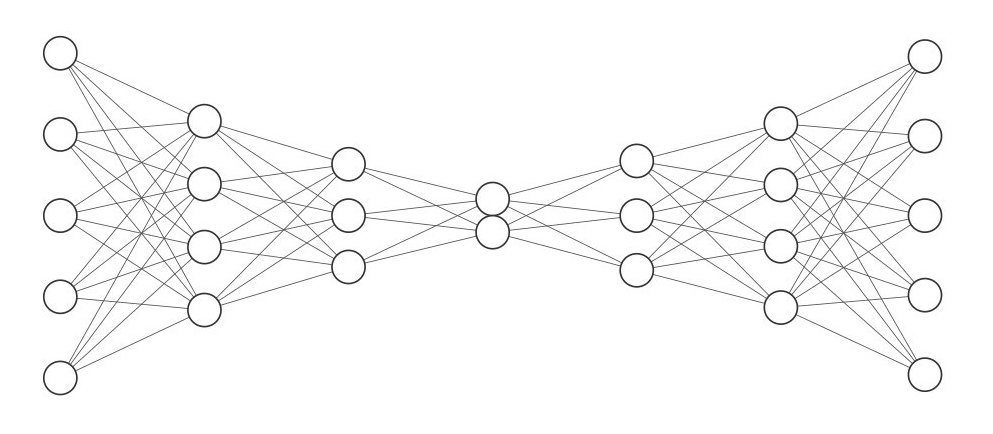
\includegraphics[width=\linewidth]{autoencoder}
      \caption{An autoencoding neural network with input and output $x, y\in \R^5$. The five hidden layers have dimensions $4$, $3$, $2$, $3$ and $4$ respectively. Hence, the bottleneck dimension is $2$ in this example. The graphic was generated with http://alexlenail.me/NN-SVG/index.html}\label{autoencoder}
	\end{minipage}
\end{center}
\end{figure}


If we divide the autoencoding structure as described above, we firstly obtain the encoder as we can see in figure \ref{img_encoder} or formally defined as follows.

\begin{definition}\label{def_encoder}
Let $\T$ be a parameter space and $\t \in \T$ a set of parameters, $L\in \N$ and $d_1,\ldots, d_L\in\N$. Let further $\f$ be an activation function and $f_{\f,L,\t}$ a neural network.\\
If the neural network $f_{\f,L,\t}$ fulfils the condition $n_i= d_1 \geq \ldots \geq d_L = n_o$ with $n_i, n_o \in \N$ being the input and output dimensions respectively, then we speak of an \textbf{encoding neural network} (or short: \textbf{encoder}) and denote it as $f_e$.
\end{definition}


\begin{figure}
\begin{center}
   \begin{minipage}[b]{0.9\linewidth}
      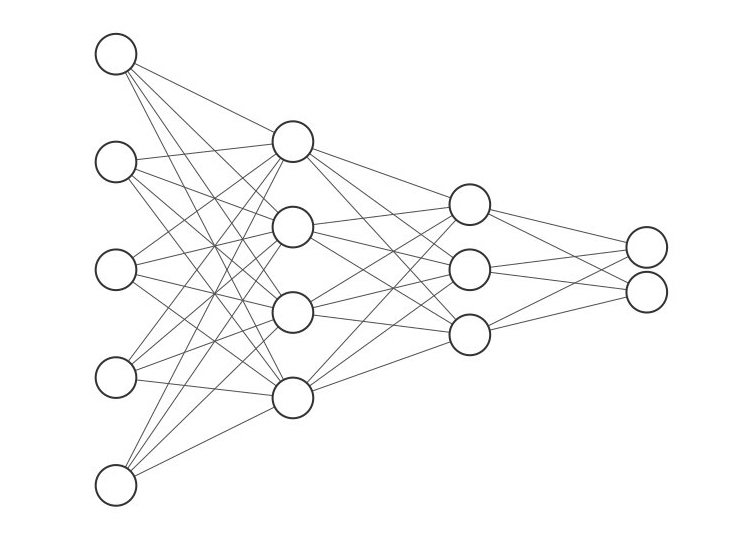
\includegraphics[width=\linewidth]{encoder}
      \caption{An encoding neural network with input $x\in \R^5$ and output $y \in \R^2$. The two hidden layers have dimensions $4$ and $3$. Hence, the encoder reduces the data dimensionality from $5$ to $2$ dimension. The graphic was generated with http://alexlenail.me/NN-SVG/index.html}\label{img_encoder}
	\end{minipage}
\end{center}
\end{figure}


For the second part of the divided autoencoding structure, we obtain the decoder as we can see in figure \ref{img_decoder}. We can define this architecture analogously to the encoder in definition \ref{def_encoder}.


\begin{definition}\label{def_decoder}
Let $\T$ be a parameter space and $\t \in \T$ a parameter, $L\in \N$ and $d_1,\ldots, d_L\in\N$. Let further $\f$ be an activation function and $f_{\f,L,\t}$ a neural network.\\
If the neural network $f_{\f,L,\t}$ fulfils the condition $n_i= d_1 \leq \ldots \leq d_L = n_o$ with $n_i, n_o \in \N$ being the input and output dimensions respectively, then we speak of an \textbf{decoding neural network} (or short: \textbf{decoder}).
\end{definition}


\begin{figure}
\begin{center}
   \begin{minipage}[b]{0.9\linewidth}
      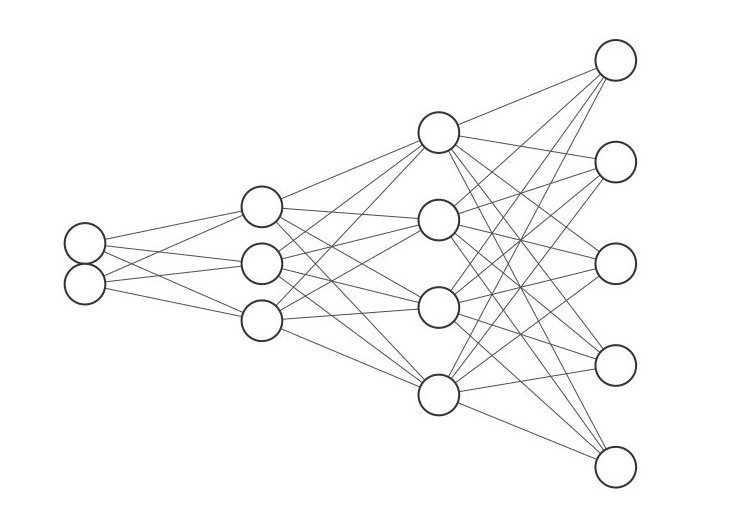
\includegraphics[width=\linewidth]{decoder}
      \caption{A decoding neural network with input $x\in \R^2$ and output $y \in \R^5$. The two hidden layers have dimensions $3$ and $4$. Hence, the decoder expands the data dimensionality from $2$ to $5$ dimensions. The graphic was generated with http://alexlenail.me/NN-SVG/index.html}\label{img_decoder}
	\end{minipage}
\end{center}
\end{figure}

Before combining the encoding and the decoding structure to obtain the autoencoding neural network, we need to consider the following technicality first.

\begin{lemma}\label{lemma:composition_of_nns}
Let $f_1, f_2$ be two neural networks of depths $L_1, L_2 \in \N$ with parameters $\t_1, \t_2 \in \T$, where $\T$ is an arbitrary parameter space. Furthermore, let the dimensions of each layer be $d_1, \ldots, d_{L_1} \in \N$ of $f_1$ and $\tilde{d}_1, \ldots, \tilde{d}_{L_2} \in \N$ of $f_2$. Additionally, let $d_{L_1} = \tilde{d}_1$.\\
Then their composition $f_2\circ f_1$ is a neural network of depth $L_1 + L_2$ with parameters $(\t_1, \t_2)$.
\end{lemma}

\begin{proof}
Since $f_1$ is a neural network of depth $L_1$ with parameters $\t_1$, its architecture looks like
\begin{align}\label{nn_1}
f_1 (x) = H_{L_1} \circ H_{L_1-1} \circ \ldots H_{2} \circ H_1 (x),\qquad x \in \R^{d_1}.
\end{align}
Analogously, we can write $f_2$ as
\begin{align}\label{nn_2}
f_2 (y) = \tilde{H}_{L_2} \circ \tilde{H}_{L_2-1} \circ \ldots \tilde{H}_{2} \circ \tilde{H}_1 (y), \qquad y \in \R^{\tilde{d}_1}.
\end{align}
Since we assumed that the output dimension $d_{L_1}$ of the neural network $f_1$ is equal to the input dimension $\tilde{d}_1$ of the neural network $f_2$, we can consider the result of \eqref{nn_1} as input for \eqref{nn_2}
\begin{align*}
y &\coloneqq H_{L_1} \circ H_{L_1-1} \circ \ldots H_{2} \circ H_1 (x), \qquad x \in \R^{d_1}.
\end{align*}
Hence, we obtain
\begin{align}\label{nn_comp}
f_2 (y) &= \tilde{H}_{L_2} \circ \tilde{H}_{L_2-1} \circ \ldots \tilde{H}_{2} \circ \tilde{H}_1 (y),\nonumber\\
f_2\left(f_1\left(x\right)\right)  &= \tilde{H}_{L_2} \circ \tilde{H}_{L_2-1} \circ \ldots \tilde{H}_{2} \circ \tilde{H}_1 \left( H_{L_1} \circ H_{L_1-1} \circ \ldots H_{2} \circ H_1 (x) \right),\nonumber\\
f_2\left(f_1\left(x\right)\right)  &= \tilde{H}_{L_2} \circ \tilde{H}_{L_2-1} \circ \ldots \tilde{H}_{2} \circ \tilde{H}_1 \circ H_{L_1} \circ H_{L_1-1} \circ \ldots H_{2} \circ H_1 (x), \qquad x \in \R^{d_1}.
\end{align}
Therefore, from \eqref{nn_comp} follows that the composition $f_2 \circ f_1$ is a neural network of depth $L_1 + L_2$.\\
Lastly, we consider the parameters $\t$ of the neural network $f_2 \circ f_1$. Since the parameters of a neural network were defined as $\t = (\t_1,\ldots, \t_L)$, where each entry is defined as $\t_i = (W_i, b_i)$ and denotes the weight and bias of each layer $H_i$ or $\tilde{H}_i$, respectively, we can write the parameters of both neural networks as
\begin{align*}
\t_1 &\coloneqq (\t_1, \ldots, \t_{L_1}) = \left((W_1, b_1),\ldots, (W_{L_1}, b_{L_1}) \right),\\
\t_2 &\coloneqq (\tilde{\t}_1, \ldots, \tilde{\t}_{L_2}) = \left((\tilde{W}_1, \tilde{b}_1),\ldots, (\tilde{W}_{L_2}, \tilde{b}_{L_2}) \right).
\end{align*}
Hence, the composition $f_2\circ f_1$ has the parameters
\begin{align*}
\t  &= \left((W_1, b_1),\ldots, (W_{L_1}, b_{L_1}), (\tilde{W}_1, \tilde{b}_1),\ldots, (\tilde{W}_{L_2}, \tilde{b}_{L_2})  \right)\\
&= \left(\t_1,\ldots \t_{L_1}, \tilde{\t}_1, \ldots, \tilde{\t}_{L_2} \right) \eqqcolon \left(\t_1,\t_2 \right).
\end{align*}
\end{proof}


Lemma \ref{lemma:composition_of_nns} allows us to consider a modern approach to neural networks, a so called modular approach. Essentially, we consider entire structures like the encoding and the decoding neural network as a self-contained module. These modules can now easily be put together by considering them in series. This is very useful in practice, since modern neural networks consist of thousands of layers and thus billions of parameters. Considering a modular approach one can therefore divide the whole neural network and tune each module separately.


\begin{theorem}
Let $\T$ be a parameter space, $N\in \N$ and $L_1,\ldots,L_N\in \N$. Furthermore, let $f_1,\ldots,f_N$ be neural networks with parameters $\t_1,\ldots,\t_N\in\T$ and depths $L_1,\ldots,L_N$, respectively. Lastly, let the output dimension of $f_i$ match the input dimension of $f_{i+1}$ for all $i\in\{1,\ldots,N-1\}$.\\
Then the composition
\begin{align*}
f \coloneqq f_{N} \circ f_{N-1} \circ \ldots \circ f_1,
\end{align*}
is a neural network with parameters $\t = (\t_1,\ldots\t_N)$ of depth $L = L_1 + \ldots + L_N$.
\end{theorem}


\begin{proof}
Applying lemma \ref{lemma:composition_of_nns} to $f_1$ and $f_2$ yields the composed neural network $f^{(1)} \coloneqq f_2 \circ f_1$ with parameters $\t^{(1)} \coloneqq (\t_1, \t_2)$ and depth $L^{(1)}\coloneqq L_1 + L_2$.\\
If we now apply lemma \ref{lemma:composition_of_nns} once again to $f^{(1)}$ and $f_3$, we receive $f^{(2)} \coloneqq f_3 \circ f^{(1)}$ with parameters $\t^{(2)} \coloneqq (\t^{(1)}, \t_3) = (\t_1, \t_2, \t_3)$ and depth $L^{(2)}\coloneqq L^{(1)} + L_3 = L_1 + L_2 + L_3$.\\
We realize, that iteratively applying lemma \ref{lemma:composition_of_nns} yields  after $N-1$ applications
\begin{align*}
f^{(N-1)} &= f_{N} \circ f_{N-1} \circ \ldots \circ f_1,\\
\t^{(N-1)}&= \left(\t_1, \ldots, \t_N \right),\\
L^{(N-1)} &= \sum_{i=1}^{N-1} L_i.
\end{align*}
Therefore the assertion is proven.
\end{proof}


\begin{definition}\label{def_autoencoder}
Let $f_e$ and $f_d$ be an encoding and a decoding neural network with input dimension $n_i$ in $\N$ and output of the encoding neural network $n_b$ in $\N$, that we will refer to as \textbf{bottleneck} of the autoencoding neural network.
Then we define an \textbf{autoencoding neural network} $f_a$ as the composition
\begin{align*}
f_a: \R^{n_i} &\to \R^{n_i},\\
x &\mapsto \left(f_d \circ f_e \right)(x).
\end{align*}
\end{definition}

\begin{remark}
Let $f_e$ and $f_d$ be an encoding and a decoding neural network as in definition \ref{def_autoencoder}. Then the composition $f_d \circ f_e$ is indeed a neural network, following from lemma \ref{lemma:composition_of_nns}.
\end{remark}


\section{Training of autoencoders}

When tackling the question of how to train an autoencoding neural network, we realize that in contrast to regular neural networks, where we compare the output of the neural network to a label, in the current setting we can compare the input data to the computed output, since the goal of an autoencoding neural network ultimately is to alter and reconstruct images. In other words, we approach this optimization problem in an unsupervised learning setting. This forces us to consider slightly different loss functions than in the supervised learning setting.


\begin{definition}
Let $X, Y$ be Banach spaces representing the input and output space, respectively.\\
Then a continuous function defined as
\begin{align*}
L:X\times Y &\to \R,\\
\left(x, p(x)\right) &\mapsto L\left(x, p(x)\right),
\end{align*}
is called \textbf{unsupervised loss function}.
\end{definition}


There are multiple important loss functions in computer vision. We will consider a couple of those in the following example. For further reading please take a look at \cite{foster2022generative}


\begin{example}
Let $\O$ be a pixel domain with resolution $(M,N)$ and $d$ the number of channels. Furthermore, let $f$ be a neural network with arbitrary but fixed architecture.\\
Then the following functions are loss functions operating on images.
\begin{mydescription}{\widthof{\textbf{Binary Cross-Entropy (BCE)}}}
\item[\textbf{Mean Squared Error (MSE)}] \begin{align*}
\MSE(\p, f(\p)) = \sum_{i=1}^{M}\sum_{j=1}^{N}\left\|\p_{ij} - f(\p)_{ij}\right\|^2,
\end{align*}
\item[\textbf{Binary Cross-Entropy (BCE)}]
\begin{align*}
\BCE(\p, f(\p)) = - \frac{1}{MN}\sum_{i=1}^{M}\sum_{j=1}^{N} \biggl(&\p_{ij} \log\left(f\left(\p\right)_{ij}\right)\\ + \bigl(1-&\p_{ij}\bigr)\log\left(1 - f\left(\p\right)_{ij}\right)\biggr),
\end{align*}
\end{mydescription}
where $\p$ denotes an image defined on $\P_{\O}$.
\end{example}


\begin{remark}
The Binary Cross-Entropy loss function is usually used for binary classification problems. However, it still works in computer vision.
\end{remark}


\section{Applications}

In this section we want to train a couple of own autoencoding neural networks on the MNIST dataset - a dataset consisting of handwritten digits. Lastly, we will consider a composition of MNIST images in order to simulate a scenario that will allow the Duckeneers GmbH to generate new data. We will consider some various architectures of neural networks and visualise the results in a comprehensible manner.\\
Firstly, we want to consider the most simple architecture, a fully connected linear neural network.

\begin{definition}\label{def_linear_encoder}
Let $\T$ be an arbitrary parameter space, $L\in \N$ and $d_1,\ldots,d_L \in \N$. Furthermore, let $\f$ be an arbitrary activation function.\\
Then an encoding neural network, where each layer $H_1,\ldots, H_L$ is defined as
\begin{align*}
H_i(x) = \hat{\f}(W_ix + b_i), \qquad x \in \R^{d_i}, i \in \{1,\ldots, L\},
\end{align*}
where $\t_i(W_i, b_i)\in\T$ are the parameters of the $i$-th layer, see \eqref{eq_linear_layer}. Such a decoding neural network is called a \textbf{linear encoder}.
\end{definition}

Analogously, we define a linear decoding neural network.

\begin{definition}\label{def_linear_decoder}
Let $\T$ be an arbitrary parameter space, $L\in \N$ and $d_1,\ldots,d_L \in \N$. Furthermore, let $\f$ be an arbitrary activation function.\\
Then a decoding neural network, where each layer $H_1,\ldots, H_L$ is defined as
\begin{align*}
H_i(x) = \hat{\f}(W_ix + b_i), \qquad x \in \R^{d_i}, i \in \{1,\ldots, L\},
\end{align*}
where $\t_i=(W_i, b_i)\in\T$ are the parameters of the $i$-th layer $H_i$, see \eqref{eq_linear_layer}. Such a decoding neural network is called a \textbf{linear decoder}.
\end{definition}


With the definitions of the linear encoder and linear decoder, we now can define a linear autoencoder.


\begin{definition}
Let $f_e$ and $f_d$ be a linear encoder and a linear decoder. Then a \textbf{linear autoencoder} $f_{\text{lin}}$ is defined as the composition
\begin{align*}
f_{\text{lin}} \coloneqq f_d \circ f_e.
\end{align*}
\end{definition}

Before considering specific examples on the MNIST dataset, we need to consider some properties of the said dataset first.

\begin{proposition}\label{def:mnist}
The MNIST dataset $\D$ consists of greyscale images with a resolution of $(28,28)$. Hence, the images are defined on the pixel domain $\O$ of $\D$ with $\O=\{1,\ldots,28\}\times\{1,\ldots,28\}$ with only one channel.
\end{proposition}

Now, let us take a look at a specific example of a linear autoencoder defined on the MNIST dataset.

\begin{algorithm}
Let the input and output dimensions be $n_i, n_o \in\N$. Furthermore, let the encoder and the decoder have $k$ hidden layers with dimensions $n_1, n_2,\ldots, n_k\in\N$ with bottleneck $n_b\N$.\\
Let the chosen optimizer be ADAM first and afterwards be AMSGrad with a learning rate $\g=\num{3e-4}$ and the MSE loss function. We will perform the training on $10.000$ epochs with a batch size of $512$.
\caption{Linear Autoencoder}\label{alg:linear_AE_2d}
\begin{algorithmic}[1]
\Require $\g \gets \num{3e-4}$
\For{epoch in $\{1,\ldots, 10.000\}$}
	\For{image in batch}
		\State image = image.reshape(784) \Comment{Convert the image from matrix to array.}
	    \State encoded = encoder(image) \Comment{Encode the image onto latent space.}
		\State reconstructed = decoder(encoded) \Comment{Decode the encoded image.}
    	\State loss = MSE(reconstructed, image) \Comment{Compare the output to the input.}
	    \State optimization(loss, $\g$) \Comment{Perform an optimization step.}
    \EndFor
\EndFor
\end{algorithmic}
\end{algorithm}


Let's take a look at the trained autoencoders using the ADAM and the AMSGrad optimizer. In figure \ref{fig:linear_AE_2d_latent} we can see the latent space of the models. Furthermore, in figure \ref{fig:linear_AE_2d_inference} we can see ten reconstructions for each of the ten digits. The training progresses are illustrated in figure \ref{fig:linear_AE_2d_training_progress}.


\begin{figure}
\begin{center}
   \begin{minipage}[b]{0.49\linewidth}
      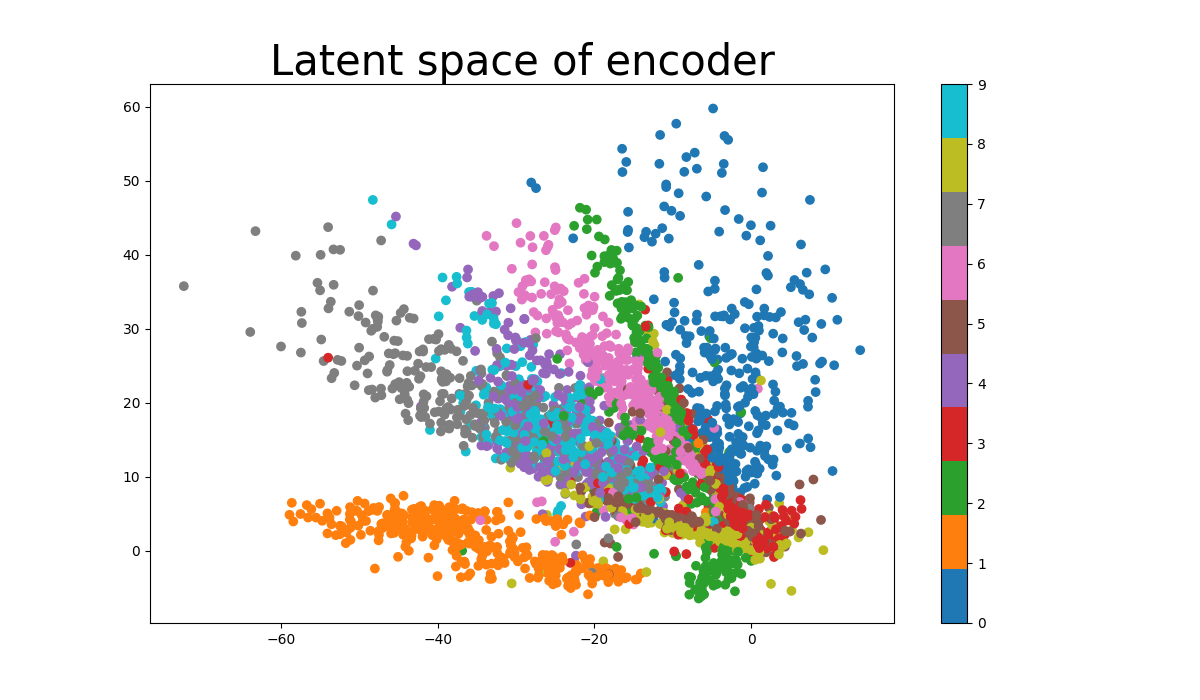
\includegraphics[width=\linewidth]{linear_AE_2d_adam_latent}
	\end{minipage}
	\begin{minipage}[b]{0.49\linewidth}
      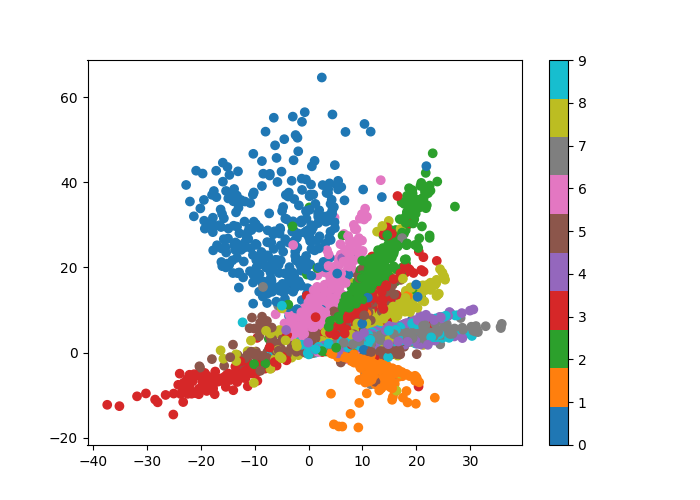
\includegraphics[width=\linewidth]{linear_AE_2d_amsgrad_latent}
	\end{minipage}
\end{center}
\caption{The figure illustrates the latent space of the linear autoencoder with bottleneck $n_b=2$ optimized with an ADAM optimizer (left) and an AMSGrad optimizer (right). Each dot is one encoded image of a digit. The color and the corresponding color map represent the digit that was encoded.}\label{fig:linear_AE_2d_latent}
\end{figure}


\begin{figure}
\begin{center}
   \begin{minipage}[b]{0.49\linewidth}
      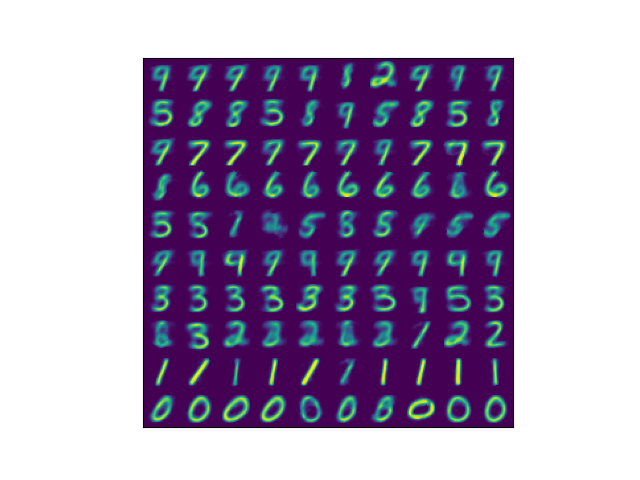
\includegraphics[width=\linewidth]{linear_AE_2d_adam_inference}
	\end{minipage}
   \begin{minipage}[b]{0.49\linewidth}
      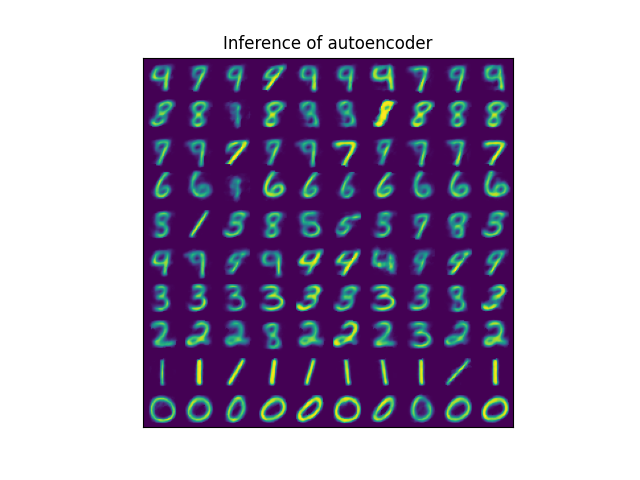
\includegraphics[width=\linewidth]{linear_AE_2d_amsgrad_inference}
	\end{minipage}
\end{center}
\caption{The figure illustrates the inference of the linear autoencoder with bottleneck $n_b=2$ optimized with an ADAM optimizer (left) and an AMSGrad optimizer (right). The inference are ten reconstructed images for each of the ten digits.}\label{fig:linear_AE_2d_inference}
\end{figure}


\begin{figure}
\begin{center}
   \begin{minipage}[b]{0.49\linewidth}
      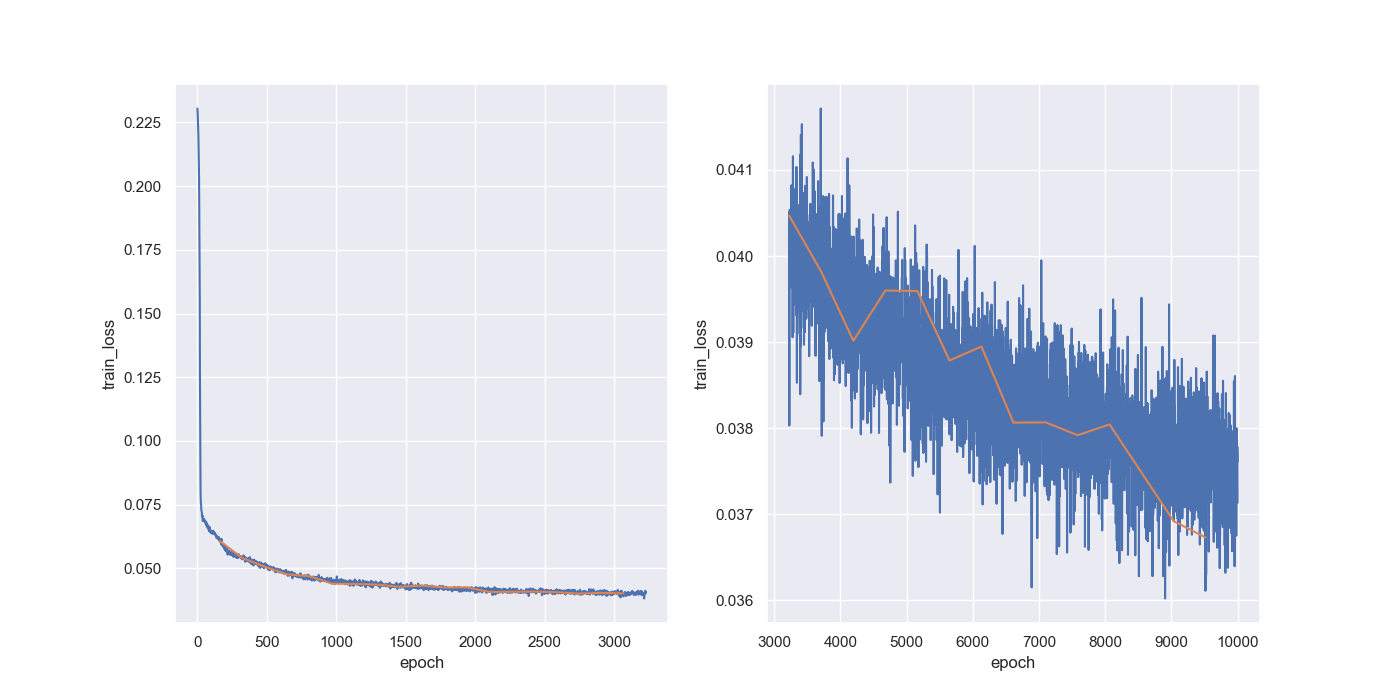
\includegraphics[width=\linewidth]{linear_AE_2d_adam_training_progress}
	\end{minipage}
   \begin{minipage}[b]{0.49\linewidth}
      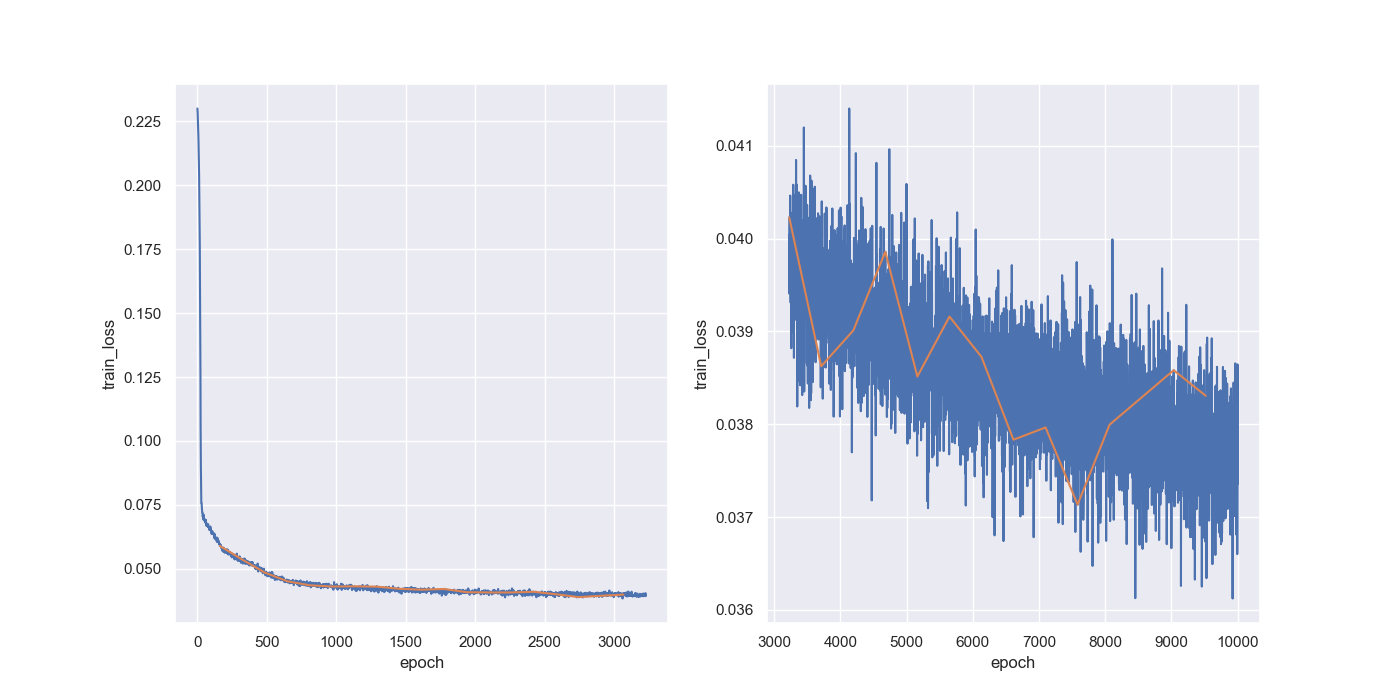
\includegraphics[width=\linewidth]{linear_AE_2d_amsgrad_training_progress}
	\end{minipage}
\end{center}
\caption{The figure illustrates the training progresses of the linear autoencoder with bottleneck $n_b=2$ optimized with an ADAM optimizer (left) and an AMSGrad optimizer (right) with epochs on one axis and corresponding training loss on the other axis.}\label{fig:linear_AE_2d_training_progress}
\end{figure}

\iffalse



Now, let's consider another latent dimension, resulting in $3$ dimensions. This allows the neural network to save more information upon encoding the data and hence, it should be able to perform better reconstructions. However, it makes visualising the latent space a bit more difficult. In figure \ref{fig:linear_AE_3d_adam_latent} we can see the latent space of the autoencoder from two different perspectives trained with the ADAM optimizer and in figure \ref{fig:linear_AE_3d_amsgrad_latent} with the AMSGrad optimizer. Furthermore, in figure \ref{fig:linear_AE_3d_inference} we can see ten reconstructions for each of the ten digits. The training progress is illustrated in figure ref{fig:linear_AE_3d_training_progress}.

\begin{figure}
\begin{center}
   \begin{minipage}[b]{0.45\linewidth}
      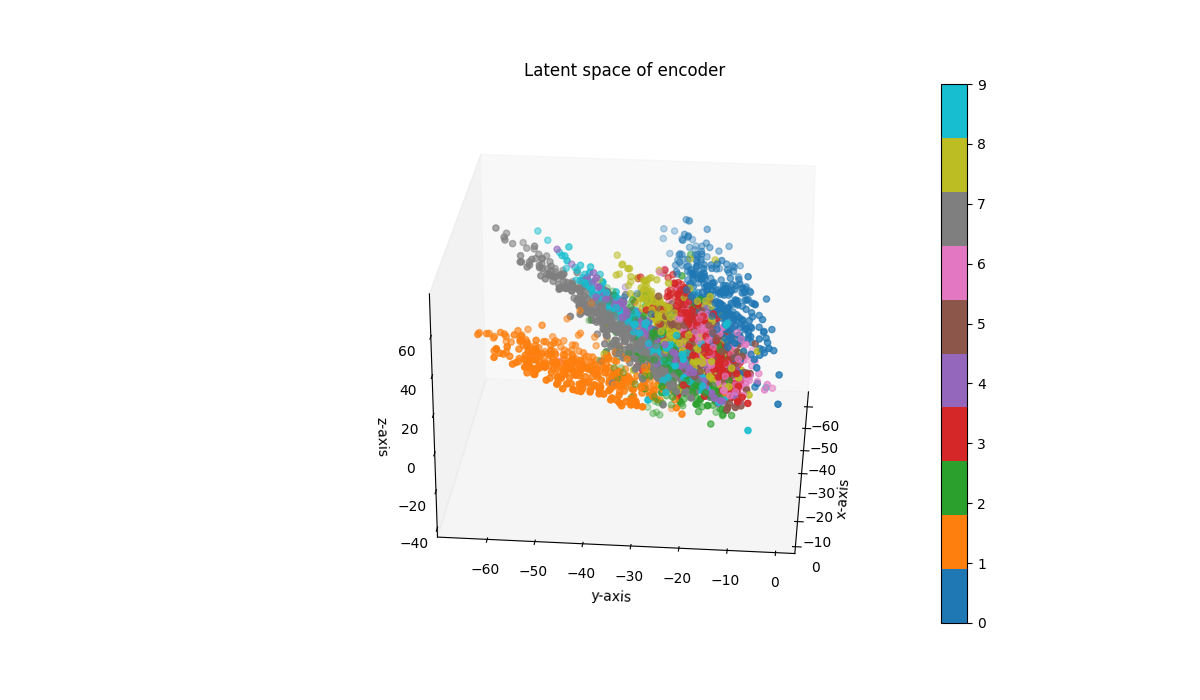
\includegraphics[width=\linewidth]{linear_AE_3d_adam_latent_1}
	\end{minipage}
	\begin{minipage}[b]{0.45\linewidth}
      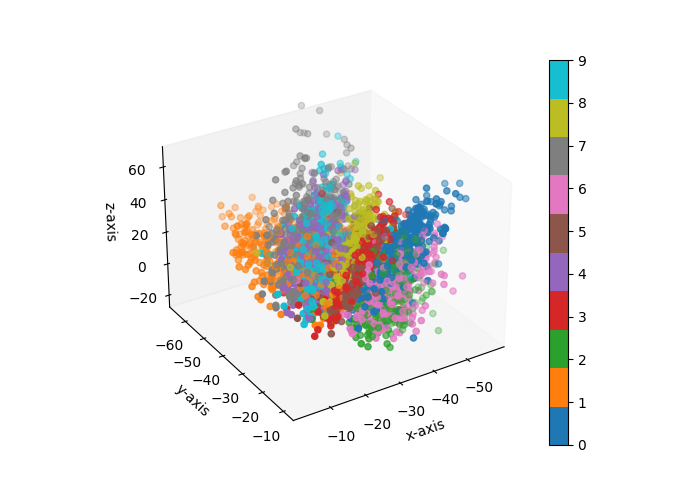
\includegraphics[width=\linewidth]{linear_AE_3d_adam_latent_2}
	\end{minipage}
\end{center}
\caption{The figure illustrates the latent space of the linear autoencoder with bottleneck $n_b=3$ optimized with an ADAM optimizer from two different perspectives. Each dot is one encoded image of a digit. The color and the corresponding color map represent the digit that was encoded.}\label{fig:linear_AE_3d_adam_latent}
\end{figure}

\begin{figure}
\begin{center}
   \begin{minipage}[b]{0.45\linewidth}
      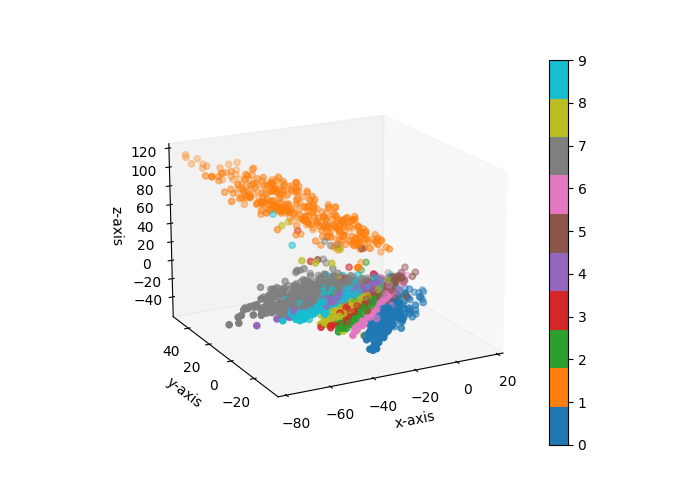
\includegraphics[width=\linewidth]{linear_AE_3d_amsgrad_latent_1}
	\end{minipage}
	\begin{minipage}[b]{0.45\linewidth}
      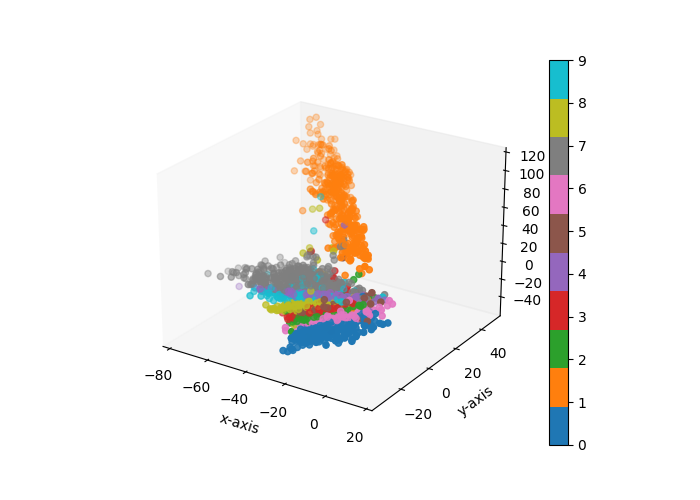
\includegraphics[width=\linewidth]{linear_AE_3d_amsgrad_latent_2}
	\end{minipage}
\end{center}
\caption{The figure illustrates the latent space of the linear autoencoder with bottleneck $n_b=3$ optimized with an AMSGrad optimizer from two different perspectives. Each dot is one encoded image of a digit. The color and the corresponding color map represent the digit that was encoded.}\label{fig:linear_AE_3d_amsgrad_latent}
\end{figure}


\begin{figure}
\begin{center}
   \begin{minipage}[b]{0.45\linewidth}
      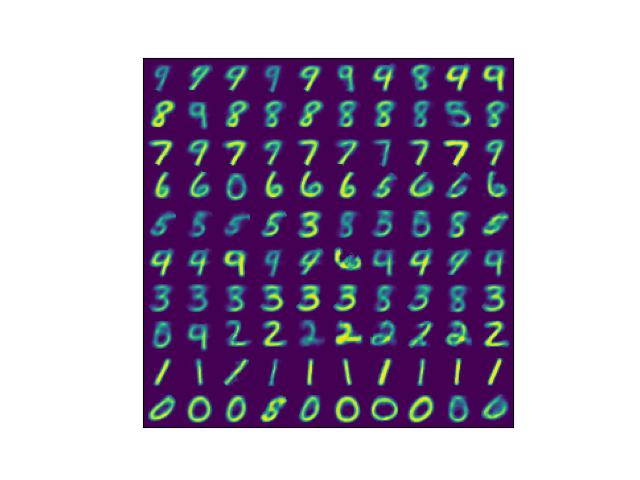
\includegraphics[width=\linewidth]{linear_AE_3d_adam_inference}
	\end{minipage}
   \begin{minipage}[b]{0.45\linewidth}
      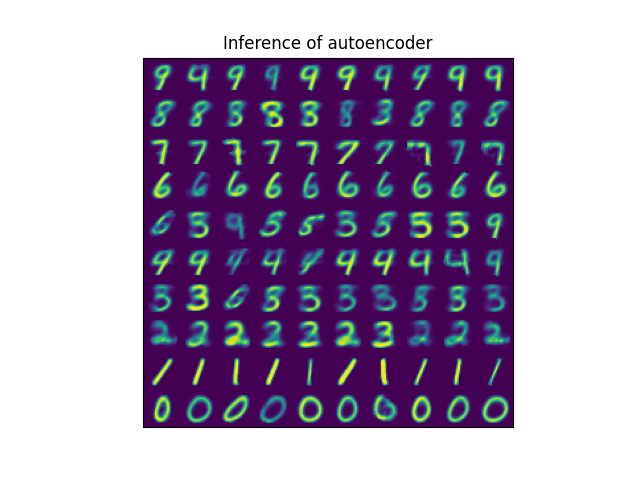
\includegraphics[width=\linewidth]{linear_AE_3d_amsgrad_inference}
	\end{minipage}
\end{center}
The figure illustrates the inference of the linear autoencoder with bottleneck $n_b=3$ optimized with an ADAM optimizer (left) and an AMSGrad optimizer (right). The inference are ten reconstructed images for each of the ten digits.\label{fig:linear_AE_3d_inference}
\end{figure}


\begin{figure}
\begin{center}
   \begin{minipage}[b]{0.45\linewidth}
      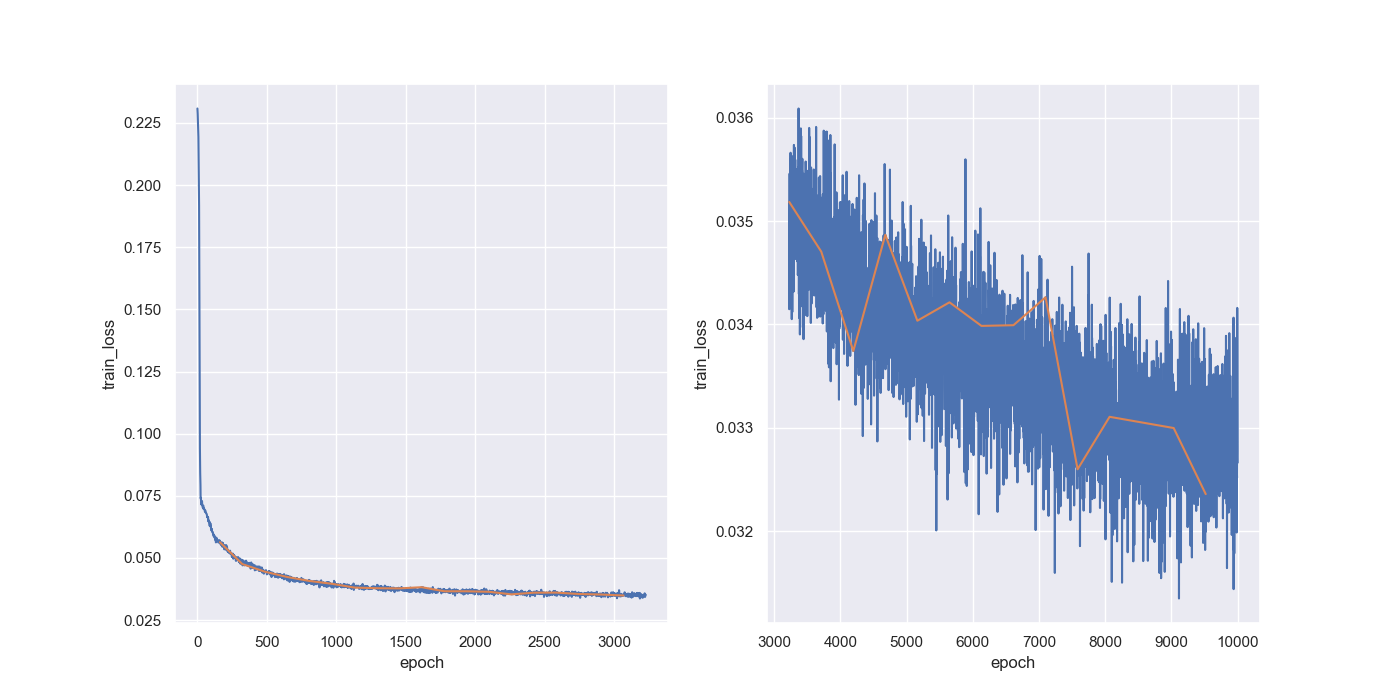
\includegraphics[width=\linewidth]{linear_AE_3d_adam_training_progress}
	\end{minipage}
	\begin{minipage}[b]{0.45\linewidth}
      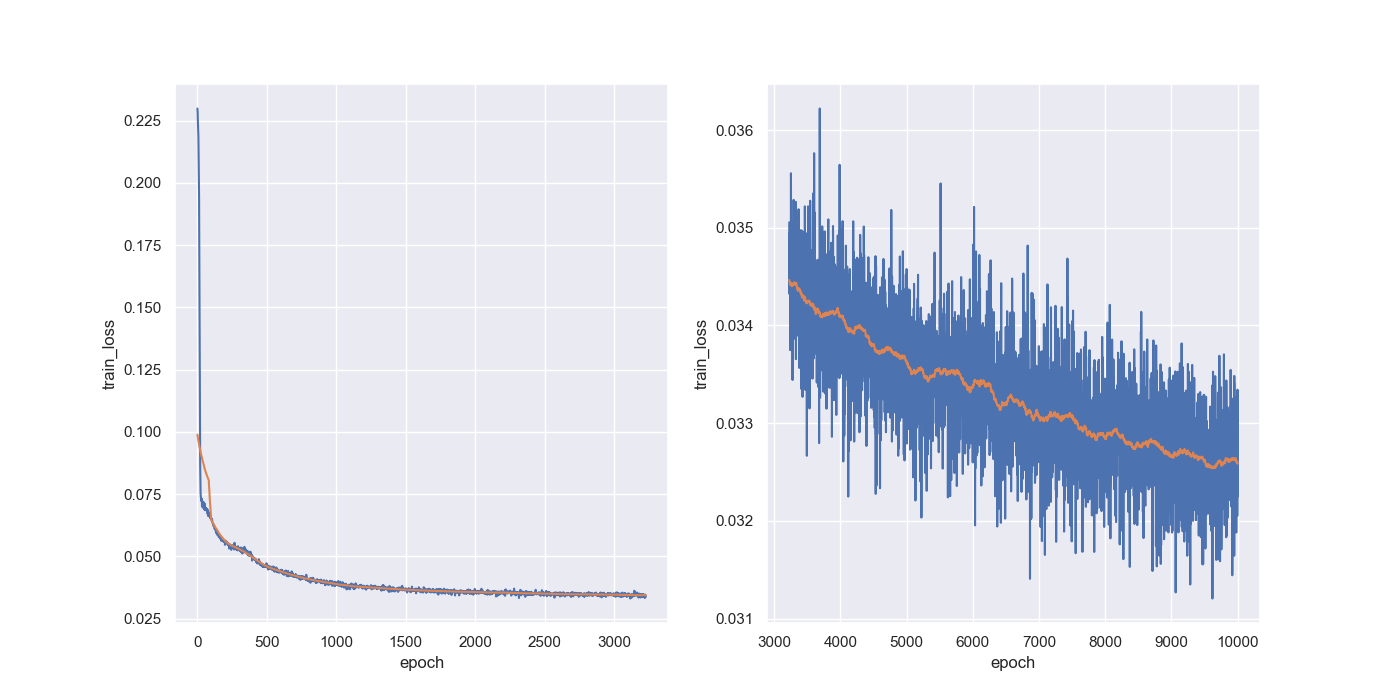
\includegraphics[width=\linewidth]{linear_AE_3d_amsgrad_training_progress}
	\end{minipage}
\end{center}
\caption{The figure illustrates the training progresses of the linear autoencoder with bottleneck $n_b=3$ optimized with an ADAM optimizer (left) and an AMSGrad optimizer (right) with epochs on one axis and corresponding training loss on the other axis.}\label{fig:linear_AE_2d_training_progress}
\end{figure}

\fi
